%----------------------------------------------------------------------------------------
\addtocounter{framenumber}{-1}
\begin{frame}
\vfill
The method works properly for the laminar case, but what happens for turbulent problems?
\vfill
\end{frame}
%----------------------------------------------------------------------------------------
\begin{frame}
 \frametitle{TGV {\small Taylor-Green Vortex flow}}
 \textbf{Effect of the grad-div term  $ (\tau_c\nabla\cdot\u,\nabla\cdot\v) $:} (coarse mesh)
 \vspace*{-0.1cm}
 \only<1-3>{
   \begin{figure}
     \centering	
     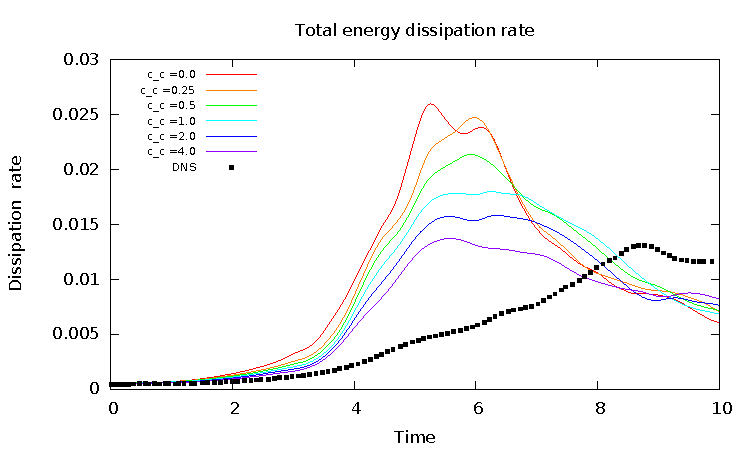
\includegraphics[width=0.75\textwidth]{Figures/TGV_OSS_ISS_tauc_tot.pdf}
     \vspace*{-0.3cm}
     \caption{Total energy dissipation rate}
   \end{figure}}
 \only<4-5>{
    \begin{figure}
      \centering	
      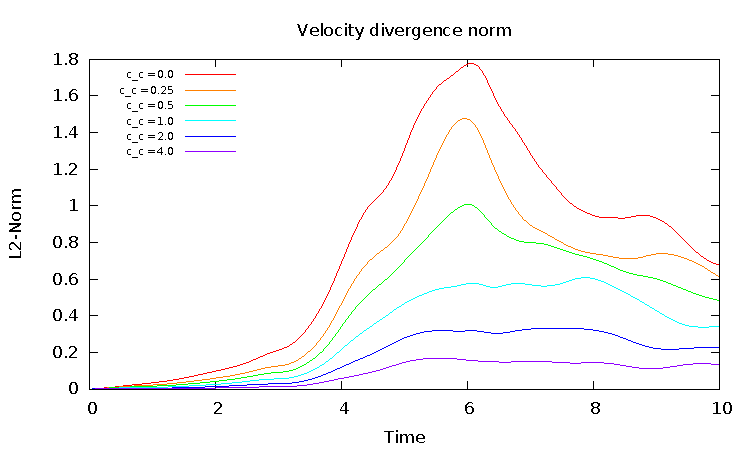
\includegraphics[width=0.75\textwidth]{Figures/TGV_OSS_ISS_tauc_div.pdf}
      \vspace*{-0.3cm}
      \caption{$\|\nabla\cdot\u\|$}
    \end{figure}}  
 \only<6->{
   \begin{figure}
     \centering	
     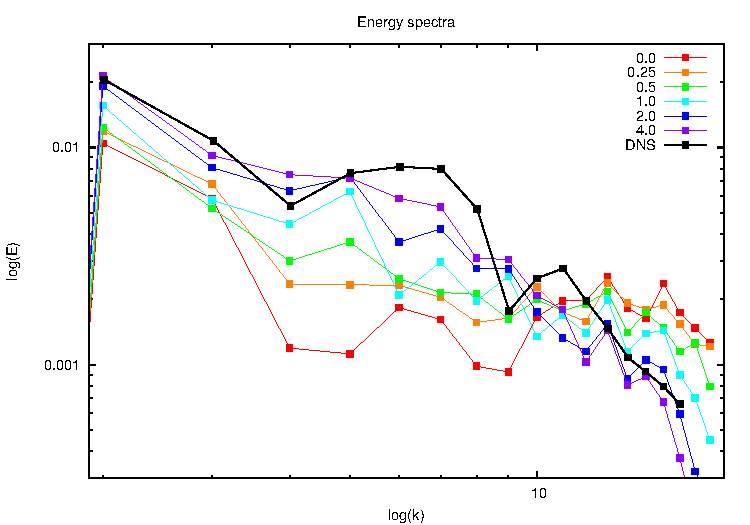
\includegraphics[width=0.65\textwidth]{Figures/TGV_OSS_ISS_tauc_spe.pdf}
     \vspace*{-0.3cm}
     \caption{Energy spectra}
   \end{figure}}
 \begin{overlayarea}{\textwidth}{1.5cm}
 \vspace*{-0.5cm}
 \only<2-3>{
 \begin{itemize}
   	\item \alert<2>{Bad results} when $ c_c\rightarrow0 $
   	\only<3>{\item Best option \alert<3>{$ c_c=4.0 $}}
 \end{itemize}}
 \only<5>{
 \begin{itemize}
   	 \item \alert<5>{Incompressibility constraint not satisfied}
 \end{itemize}}
 \only<7->{
 \begin{itemize}
   	\item \alert<7>{Over-dissipation} on the \alert<7>{large scales} when $ c_c\rightarrow0 $
   	\only<8>{\item \alert<8>{Infra-dissipation} on the \alert<8>{small scales} when $ c_c\rightarrow0 $}
 \end{itemize}}
 \end{overlayarea}
\end{frame}